\documentclass[3p, authoryear]{elsarticle} %review=doublespace preprint=single 5p=2 column
%%% Begin My package additions %%%%%%%%%%%%%%%%%%%
\usepackage[hyphens]{url}

  \journal{Findings} % Sets Journal name


\usepackage{lineno} % add
\providecommand{\tightlist}{%
  \setlength{\itemsep}{0pt}\setlength{\parskip}{0pt}}

\usepackage{graphicx}
%%%%%%%%%%%%%%%% end my additions to header

\usepackage[T1]{fontenc}
\usepackage{lmodern}
\usepackage{amssymb,amsmath}
\usepackage{ifxetex,ifluatex}
\usepackage{fixltx2e} % provides \textsubscript
% use upquote if available, for straight quotes in verbatim environments
\IfFileExists{upquote.sty}{\usepackage{upquote}}{}
\ifnum 0\ifxetex 1\fi\ifluatex 1\fi=0 % if pdftex
  \usepackage[utf8]{inputenc}
\else % if luatex or xelatex
  \usepackage{fontspec}
  \ifxetex
    \usepackage{xltxtra,xunicode}
  \fi
  \defaultfontfeatures{Mapping=tex-text,Scale=MatchLowercase}
  \newcommand{\euro}{€}
\fi
% use microtype if available
\IfFileExists{microtype.sty}{\usepackage{microtype}}{}
\usepackage{natbib}
\bibliographystyle{plainnat}
\usepackage{longtable,booktabs,array}
\usepackage{calc} % for calculating minipage widths
% Correct order of tables after \paragraph or \subparagraph
\usepackage{etoolbox}
\makeatletter
\patchcmd\longtable{\par}{\if@noskipsec\mbox{}\fi\par}{}{}
\makeatother
% Allow footnotes in longtable head/foot
\IfFileExists{footnotehyper.sty}{\usepackage{footnotehyper}}{\usepackage{footnote}}
\makesavenoteenv{longtable}
\usepackage{graphicx}
\ifxetex
  \usepackage[setpagesize=false, % page size defined by xetex
              unicode=false, % unicode breaks when used with xetex
              xetex]{hyperref}
\else
  \usepackage[unicode=true]{hyperref}
\fi
\hypersetup{breaklinks=true,
            bookmarks=true,
            pdfauthor={},
            pdftitle={Simulating Geofenced Microtransit in Salt Lake County},
            colorlinks=false,
            urlcolor=blue,
            linkcolor=magenta,
            pdfborder={0 0 0}}
\urlstyle{same}  % don't use monospace font for urls

\setcounter{secnumdepth}{5}
% Pandoc toggle for numbering sections (defaults to be off)

% Pandoc citation processing

% Pandoc header
\usepackage{booktabs}
% \usepackage{ragged2e}
\usepackage{booktabs}
\usepackage{longtable}
\usepackage{array}
\usepackage{multirow}
\usepackage{wrapfig}
\usepackage{float}
\usepackage{colortbl}
\usepackage{pdflscape}
\usepackage{tabu}
\usepackage{threeparttable}
\usepackage{threeparttablex}
\usepackage[normalem]{ulem}
\usepackage{makecell}
\usepackage{xcolor}



\begin{document}
\begin{frontmatter}

  \title{Simulating Geofenced Microtransit in Salt Lake County}
    \author[Brigham Young University]{Hayden Atchley}
   \ead{satchley@byu.edu} 
    \author[Brigham Young University]{Gregory Macfarlane}
   \ead{gregmacfarlane@byu.edu} 
      \address[Brigham Young University]{Civil and Construction Engineering Department, 430 Engineering Building, Provo, Utah 84602}
    
  \begin{abstract}
  A number of regions have begun operating microtransit systems to support first and last mile transit access. In this paper, we modify the ridehailing request handling algorithm in the BEAM microscopic simulation engine to accomodate geographically resetricted microstransit operations. We then examine the ridership operating characteristics for one existing and three proposed geofenced service regions in Salt Lake County, Utah. We find that the simulation generates realistic ridership statistics and wait times, subject to errors likely to be corrected with more thorough choice model calibration. We also found that expanding microtransit services to Sandy or West Jordan might be effective, but might be less so for the area near SLC International Airport.
  \end{abstract}
   \begin{keyword} Microtransit, Passive Data, Location Choice\end{keyword}
 \end{frontmatter}

\hypertarget{question}{%
\section{Question}\label{question}}

In November of 2019, Utah Transit Authority (UTA) began a partnership with Via Transportation, a private mobility company \citep{UTAreport}.
Under this partnership, UTA has supplemented its fixed-route services with on-demand shuttles hailed through a mobile application.
So-called ``microtransit'' offerings of this kind have the potential to efficiently extend UTA services into low-density areas and function as first- and last-mile services for the regular fixed-route rail and bus network.
The current microtransit service is currently only operating in southern Salt Lake County \citep{UTAonDemand}.
UTA is interested in examining if there are other areas where similar services can be effectively deployed.

In September 2020, UTA released a report detailing a possible expansion of microtransit services to other areas in Utah following the UTA on Demand pilot program \citep{UTAreport}.
19 zones were identified between Brigham City and Santaquin as areas that could potentially benefit from microtransit services.
Ridership was estimated based on number of residents and number of workers employed within each zone, as well as a mode share score that VIA developed based on their internal demand model.

We seek however to provide UTA and the Utah Department of Transportation (UDOT) with a microsimulation model they can use as a template to examine future similar projects.
We want to know how the results of such a model would compare to those of UTA's September 2020 report.
Though UTA's own report made no definitive recommendations regarding expansion of microtransit services, it may be useful in calibrating our simulation.
We also seek to use our results (possibly in conjunction with those of UTA's report) to make recommendations to UTA and UDOT regarding expansion of microtransit services.

\hypertarget{methods}{%
\section{Methods}\label{methods}}

We used BEAM (Behavior, Energy, Autonomy, and Mobility) as our model to run and calibrate our simulations. BEAM is being developed by Lawrence Berkeley National Laboratory and the UC Berkeley Institute for Transportation Studies, and is an extension to the MATSim (Multi-Agent Transportation Simulation) model \citep{beamdocs}. We created a fork of the main BEAM repository for this and other projects. One aspect of the code we developed is the ability to add geofencing, in which ridehail vehicles are constrained to a specific polygon. The version of the code we used is available at https://github.com/tscore-utc/beam/commit/b28bc396fd50db6099e9aecc54c24642feb4f74d.

As UTA already has a ridehail pilot program underway, we reached out to find the fleet size and shifts for the ridehail vehicles. Shaina Quinn, a researcher at UTA's Office of Innovative Mobility Solutions, informed us that typically 12 ridehail vehicles provide service at a time. We found the shifts on UTA's website for the service \citep{SLCSouth}. Since we didn't have information on fleet size or shifts for any scenario except the existing pilot program, we used the same values for each additional study area as well.

We first created a base scenario to model the existing pilot program. There were three other areas we wished to analyze for potential ridehail expansion: near SLC Int'l Airport, Sandy, and West Jordan. The area near the airport is planned to get ridehail service beginning December 13, 2021 \citep{Airport}, so we included that area in all scenarios except the base. A map including all of the areas is shown in Figure \ref{fig:map}.

\begin{figure}
\centering
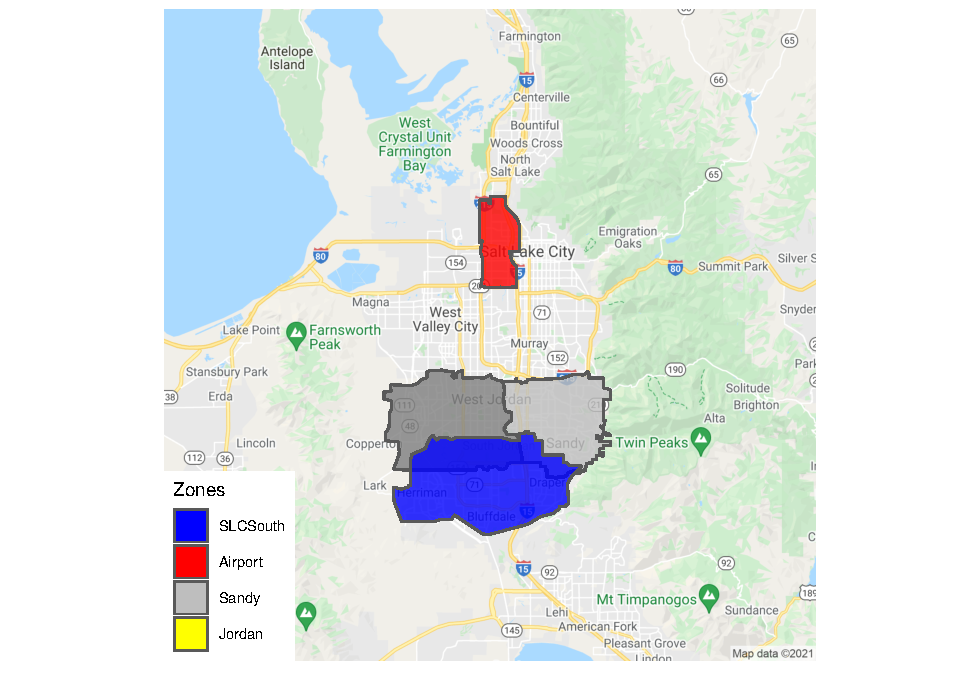
\includegraphics{microtransit-areas_files/figure-latex/map-1.pdf}
\caption{\label{fig:map}Ridehail zones in Salt Lake County.}
\end{figure}

We compared the different scenarios on several metrics, including weekday ridership, utilization (passengers/hour/vehicle), wait time, and travel time. We also compared the base scenario to the results of UTA's September 2020 report \citep{UTAreport}. Some metrics of interest from that report were average ridership, wait time, and utilization. These results are presented in Table \ref{tab:UTAOD} below.

\begin{table}[H]

\caption{\label{tab:UTAOD}UTA On Demand Report Findings}
\centering
\begin{tabular}[t]{lrrr}
\toprule
Month & Avg wkday ridership & Utilization$^{\text{a}}$ & Avg wait time\\
\midrule
\cellcolor{gray!6}{DEC} & \cellcolor{gray!6}{224.00} & \cellcolor{gray!6}{1.33} & \cellcolor{gray!6}{9.00}\\
JAN & 334.00 & 2.00 & 11.00\\
\cellcolor{gray!6}{FEB} & \cellcolor{gray!6}{392.00} & \cellcolor{gray!6}{2.31} & \cellcolor{gray!6}{12.00}\\
MAR & 316.00 & 1.88 & 11.00\\
\cellcolor{gray!6}{APR} & \cellcolor{gray!6}{275.00} & \cellcolor{gray!6}{1.52} & \cellcolor{gray!6}{10.00}\\
MAY & 105.00 & 0.67 & 8.00\\
\cellcolor{gray!6}{JUN} & \cellcolor{gray!6}{162.00} & \cellcolor{gray!6}{1.10} & \cellcolor{gray!6}{9.00}\\
JUL & 155.00 & 1.10 & 9.00\\
\cellcolor{gray!6}{AUG} & \cellcolor{gray!6}{193.00} & \cellcolor{gray!6}{1.50} & \cellcolor{gray!6}{12.00}\\
SEP & 214.00 & 1.60 & 12.00\\
\cellcolor{gray!6}{OCT} & \cellcolor{gray!6}{200.00} & \cellcolor{gray!6}{1.70} & \cellcolor{gray!6}{13.00}\\
NOV & 169.00 & 1.70 & 13.00\\
\textbf{\cellcolor{gray!6}{Average}} & \textbf{\cellcolor{gray!6}{228.25}} & \textbf{\cellcolor{gray!6}{1.53}} & \textbf{\cellcolor{gray!6}{10.75}}\\
\textbf{Average Jan--Mar} & \textbf{347.33} & \textbf{2.06} & \textbf{11.33}\\
\bottomrule
\multicolumn{4}{l}{\textsuperscript{a} Utilization is calculated as passengers per hour per vehicle}\\
\end{tabular}
\end{table}

\hypertarget{findings}{%
\section{Findings}\label{findings}}

We calculated several metrics from the output of our base (``South SL County only'') scenario and compared them with data from UTA's report on their pilot program \citep{UTAevalQ1, UTAevalQ2, UTAevalQ3, UTAevalQ4}. Much of the data in that report, however, is not necessarily representative, due to the COVID-19 pandemic and its onset in late March 2020. We also considered that the data for December was not necessarily valuable: since the service was new, people who would otherwise have used it may not have been accustomed to or even known about it. We therefore decided to use the average of the data from January through March. The comparison is given in Table \ref{tab:UTAComparison}.

\begin{table}[H]

\caption{\label{tab:UTAComparison}Comparison of Actual Pilot Program Data with Simulated Base Scenario}
\centering
\begin{tabular}[t]{lrrr}
\toprule
Scenario & Weekday Ridership & Average Wait Time (minutes) & Utilization$^{\text{a}}$\\
\midrule
\cellcolor{gray!6}{South SL County only} & \cellcolor{gray!6}{1006.00} & \cellcolor{gray!6}{5.82} & \cellcolor{gray!6}{4.14}\\
UTA Report Average Jan--Mar & 347.33 & 11.33 & 2.06\\
\bottomrule
\multicolumn{4}{l}{\textsuperscript{a} Utilization is calculated as passengers per hour per vehicle}\\
\end{tabular}
\end{table}

It is clear from this comparison that more calibration is required in order to better match the real-world data from the pilot program. There are several ways to adjust parameters and code in BEAM to achieve this calibration, and work is planned to continue on doing exactly that (though that is outside the scope of this report). However, it is encouraging to see that the simulated values are within an order of magnitude of the real-world values.

Additionally, we calculated these and other metrics for our other scenarios, and compared them. These metrics are given in Table \ref{tab:comparison}.

\begin{table}[H]

\caption{\label{tab:comparison}Comparison of Simulated Scenarios}
\centering
\resizebox{\linewidth}{!}{
\begin{tabular}[t]{lrrrrr}
\toprule
Scenario & Weekday Ridership & Ride Hail Trips & Percent of RH Trips & Average Wait Time (minutes) & Utilization$^{\text{a}}$\\
\midrule
\cellcolor{gray!6}{South SL County only} & \cellcolor{gray!6}{1006} & \cellcolor{gray!6}{930} & \cellcolor{gray!6}{1.16} & \cellcolor{gray!6}{5.82} & \cellcolor{gray!6}{4.14}\\
South SLC with Airport & 1395 & 1328 & 1.66 & 5.37 & 2.87\\
\cellcolor{gray!6}{South SLC/Airport/Sandy} & \cellcolor{gray!6}{2796} & \cellcolor{gray!6}{2473} & \cellcolor{gray!6}{3.08} & \cellcolor{gray!6}{5.77} & \cellcolor{gray!6}{3.84}\\
South SLC/Airport/West Jordan & 2620 & 2353 & 2.93 & 5.53 & 3.59\\
\bottomrule
\multicolumn{6}{l}{\textsuperscript{a} Utilization is calculated as passengers per hour per vehicle}\\
\end{tabular}}
\end{table}

These results seem to indicate that adding a ridehail zone near the airport would not have much of an effect, but adding a zone in either Sandy or West Jordan would. It's possible that the airport zone was too small to be of much use. Additionally, there is already public transit to the airport, so adding a ridehail service wouldn't necessarily provide much additional benefit. However, the other scenarios present a substantial increase in ridership, as well as percentage of trips involving a ridehail vehicle. Utilization in these scenarios on the other hand doesn't seem to improve; it may be that the fleet size needs to be adjusted to better match the demand.

Overall, these results seem to indicate that additional implementation of ridehail services would see good use, and should be seriously considered by UTA.

\hypertarget{acknowledgements}{%
\section*{Acknowledgements}\label{acknowledgements}}
\addcontentsline{toc}{section}{Acknowledgements}

We would like to thank all who have contributed to the R packages we used, notably:

\begin{itemize}
\tightlist
\item
  tidyverse (https://tidyverse.tidyverse.org/)
\item
  ggmap (https://github.com/dkahle/ggmap)
\item
  kableExtra (https://rdocumentation.org/packages/kableExtra/versions/1.3.4)
\end{itemize}

\bibliography{references.bib}


\end{document}
